%****************************************************
%	CHAPTER 3 - Dynamics
%****************************************************
\chapter{Kinematics \& Dynamics}
\label{ch:dynamics}
%====================================================
The body's dynamics are first treated as rigid, with appropriate equations derived for generic 6-DOF motion. There after, non-linear aerodynamic and inertial effects, unique to multi-body relative rotations, are investigated and incorporated into the plant's model. Finally a consolidated, quaternion based plant model is presented which is used for the later control plant development next in Chapter:\ref{ch:control}.
%====================================================
\section{Rigid Body Dynamics}
\label{sec:dynamics.rigidbody}
%====================================================
\subsection{Lagrange Derivation}
\label{subsec:dynamics.rigidbody.lagrange}
%====================================================
Fundamentally any body, rigid or otherwise, can undergo two kinds of movements, namely rotational and translation motions. Often a Lagrangian\cite{classicaldynamics,rotationrigidbody} approach for combined angular and translational movements is used to derive the differential equations of motion for each degree of freedom. The Lagrangian principle ensures that translational and rotational kinematic energies and potential energy are conserved throughout the system's trajectory progression. When combined with Euler-Rotational equations, the Euler-Lagrangian\cite{lagrange-formalism} formulation fully defines the aerospace 6-DOF equation set.
\par
Lagrangian formalism is regarded as especially useful in non-cartesian (\emph{spherical etc\ldots}) co-ordinate frames or multi-body systems. With that being said, a cartesian co-ordinate system was already defined in Section:\ref{subsec:proto.conventions.motoraxis}. Rigid body dynamics in a cartesian co-ordinate frame do lend themselves to Newtonian mechanics. The Newton-Euler or Euler-Lagrange formulations both stipulate the same resultant differential equations of motion. The Lagrangian operator, $\mathcal{L}$, is a term made up of the difference between kinetic and potential energies, $T$ and $U$ respectively. Considering some generalized path co-ordinates $\mathbf{r}(t)$, for both linear $\vec{\mathcal{E}}$ and angular $\vec{\eta}$ relative positions;
\begin{equation}\label{eq:generalpath}
\mathbf{r}(t)=\begin{bmatrix}
\vec{\mathcal{E}} & \vec{\eta}
\end{bmatrix}^T
\end{equation}
The co-ordinates in Eq:\ref{eq:generalpath} are generalized here, despite being symbols commonly used to represent linear and angular positions. The generalized co-ordinates are later be refined as Cartesian body co-ordinates with respect to the inertial frame. The Lagrangian is, by definition:
\begin{subequations}
\begin{equation}\label{eq:lagrangian.a}
\mathcal{L}(\mathbf{r},\dot{\mathbf{r}},t)=T(\mathbf{r},\dot{\mathbf{r}})-U(\mathbf{r},\dot{\mathbf{r}})
\end{equation}
Introducing a rigid body's general kinetic (angular \& linear) and potential energies, the latter being only gravitational\footnote{Here $G=\begin{bmatrix}
0&0&-9.81
\end{bmatrix}^T~m.s^{-2}$~in the Inertial frame,$\in\mathcal{F}^I$} potential energy in this case:
\begin{equation}\label{eq:lagrangian.b}
\mathcal{L}=\frac{1}{2}\dot{\vec{\mathcal{E}}}^{~T}(m)\dot{\vec{\mathcal{E}}}+\frac{1}{2}\dot{\vec{\eta}}^{~T}(\mathbb{I})\dot{\vec{\eta}}-m\vec{G}z
\end{equation}
\end{subequations}
\newpage
Noting that $\mathbb{I}$ is the inertial tensor of the body aligned w.r.t to whichever generalized reference frame is used. The Euler-Lagrange formulation equates partial derivatives of the Lagrangian to any generalized forces, $\mathbf{V}$, acting on the system. In this case the generalized forces or, more specifically a net force $\vec{F}_{net}$ and a net torque $\vec{\tau}_{net}$.
\begin{equation}\label{eq:euler-lagrange}
\frac{d}{dt}\bigg(\frac{\delta L}{\delta \dot{\mathbf{r}}}\bigg)-\frac{\delta L}{\delta \mathbf{r}} = \mathbf{V} = \begin{bmatrix}
\vec{F}_{net}\\
\vec{\tau}_{net}
\end{bmatrix}
\end{equation}
And taking the partial derivatives of Eq:\ref{eq:lagrangian.b} with respect to the path co-ordinates $\mathbf{r}$:
\begin{subequations}
\begin{equation}\label{eq:partial.a}
\frac{\delta L}{\delta \mathbf{r}}=\begin{bmatrix}
m\vec{G}_x\\
0
\end{bmatrix}
\end{equation}
\vspace{-5pt}
\begin{equation}\label{eq:partial.b}
\frac{d}{dt}\bigg(\frac{\delta L}{\delta \dot{\mathbf{r}}}\bigg)=\bigg[
m\frac{d}{dt}\dot{\vec{\mathcal{E}}} ~~~ \mathbb{I}\frac{d}{dt}\dot{\vec{\eta}}\bigg]^T
\end{equation}
\end{subequations}
Where $\vec{G}_x$ is the gravitation force in whichever reference frame ($\mathcal{F}^x$) the lagrangian is with respect to. In any generalized coordinate system a rotating vector's time derivative which, according to the Reynolds Transportation Theorem\cite{reynolds,conservationequations}, is given by:
\begin{equation}\label{eq:reynolds}
\frac{d\vec{f}}{dt_a}=\frac{d\vec{f}}{dt_b}+\vec{\omega}_{a/b}\times\vec{f}
\end{equation}
So applying that theorem (Eq:\ref{eq:reynolds}) to the partial derivatives in Eq:\ref{eq:partial.b} and further defining the generalized co-ordinates as cartesian body coordinates with respect to an inertial origin (the body frame $\mathcal{F}^b$). Noting that in Eq:\ref{eq:partial.b} the place holders used for linear ($\vec{\mathcal{E}}$) and angular positions ($\vec{\eta}$) are in a common shared frame\footnote{In this case $\vec{\eta}\not=[\phi~\theta~\psi]^T$ seeing that angular position $\vec{\eta}$ is defined in a common frame. $\vec{\eta}$ is \underline{NOT} an Euler angle set.}, and hence:
\begin{equation}
\frac{d}{dt}
\big[ \vec{\mathcal{E}} ~~ \vec{\eta} \big]^T
\equiv
\big[ \vec{\nu} ~~ \vec{\omega}\big]^T \in \mathcal{F}^b
\end{equation}
It then follows that the Lagrangian Eq:\ref{eq:lagrangian.b} changes to:
\begin{subequations}
\begin{equation}
\mathcal{L}=\frac{1}{2}\vec{\nu}^{~T}(m)\vec{\nu}+\frac{1}{2}\vec{\omega}^{~T}(\mathbb{I})\vec{\omega} -m\vec{G}_b z
\end{equation}
\vspace{-5pt}
\begin{equation}
\frac{d}{dt}\bigg(\frac{\delta L}{\delta \dot{\mathbf{r}}}\bigg)=\bigg[
m\frac{d}{dt}\vec{\nu} ~~~ \mathbb{I}\frac{d}{dt}\vec{\omega}\bigg]^T
\end{equation}
\vspace{-5pt}
\begin{equation}
\rightarrow m\frac{d}{dt}\vec{\nu}=m\dot{\vec{\nu}}+\vec{\omega}_{I/b}\times\vec{\nu}
\end{equation}
\vspace{-5pt}
\begin{equation}
\rightarrow \mathbb{I}_b \frac{d}{dt}\vec{\omega}=\mathbb{I}_b\dot{\vec{\omega}}+\vec{\omega}_{I/b}\times\mathbb{I}_b\vec{\omega}
\end{equation}
\end{subequations}
Which, when substituted back into the Euler-Lagrange formulation Eq:\ref{eq:euler-lagrange}, results in the familiar Newton-Euler equations for linear and angular differentials, both in the body frame;
\begin{subequations}\label{eq:newton}
\begin{equation}\label{eq:newton.a}
\vec{F}_{net}=m\dot{\vec{\nu}}+\vec{\omega}_b\times m \vec{\nu} - m\mathbb{R}_I^b(-\eta) \vec{G}_I
\end{equation}
\vspace{-15pt}
\begin{equation}\label{eq:newton.b}
\vec{\tau}_{net}=\mathbb{I}_b\dot{\vec{\omega}}_b+\vec{\omega}_b\times\mathbb{I}_b\vec{\omega}_b
\end{equation}
\end{subequations}
It's important to recall that $\vec{\omega}_b\not= \dot{\vec{\eta}}$ where $\vec{\eta}=[\phi~\theta~\psi]^T$, seeing that Euler Angles are defined in sequentially rotated reference frames. So then four differential equations are often used to completely describe the entire set of state derivatives, namely:
\begin{subequations}\label{eq:states}
\begin{equation}\label{eq:states.a}
\dot{\vec{\mathcal{E}}}=\mathbb{R}_b^I(-\eta)\vec{\nu}~~~~\in\mathcal{F}^I
\end{equation}
\vspace{-10pt}
\begin{equation}\label{eq:states.b}
\vec{F}_{net}=m\dot{\vec{\nu}}+\vec{\omega}_b\times m\vec{\nu} -m \mathbb{R}_I^b(-\eta)\vec{G}_I ~~~~\in\mathcal{F}^b
\end{equation}
\newpage
\begin{equation}\label{eq:states.c}
\dot{\vec{\eta}}=\Psi(\eta)\vec{\omega}_b~~~~\in\mathcal{F}^{v2},\mathcal{F}^{v1},\mathcal{F}^I
\end{equation}
\vspace{-10pt}
\begin{equation}\label{eq:states.d}
\vec{\tau}_{net}=\mathbb{I}_b\vec{\omega}_b+\vec{\omega}_b\times\mathbb{I}_b\vec{\omega}~~~~\in\mathcal{F}^b
\end{equation}
\end{subequations}
The state differentials in Eq:\ref{eq:states} can be reduced to a set of two equations. Those differentials are defined in reference frames of the state variables which they represent. The non-linear form of those equations substitutes\footnote{Originally introduced in Eq:\ref{eq:angular-rates.e}} $d\vec{\eta}/dt=\Phi(\eta)\vec{\omega}_b$ in the Lagrangian derivative, Eq:\ref{eq:partial.b}.
\begin{equation}
\frac{d}{dt}\bigg(\frac{\delta \mathcal{L}}{\delta \dot{\mathbf{r}}}\bigg)=\bigg[m\frac{d}{dt}\vec{\nu}~~~\mathbb{I}\frac{d}{dt}\dot{\vec{\eta}}\bigg]^T=\bigg[m\frac{d}{dt}\vec{\nu}~~~\mathbb{I}\frac{d}{dt}\Phi(\eta)\vec{\omega}_b\bigg]^T
\end{equation}
This only affects the angular component as the two kinetic energies are independent of one another. And so applying the differential chain rule:
\begin{equation}
\mathbb{I}\frac{d}{dt}\Phi(\eta)\dot{\vec{\omega}}_b=\mathbb{I}\big(\Phi\dot{(\eta)}\vec{\omega}_b+\Phi(\eta)\dot{\vec{\omega}}_b \big)
\end{equation}
\par
Drawing from \cite{autonomousrobotseuler} and recognizing that $\mathbb{I}$ must be transformed to the common intermediate euler axes, $\mathbb{J}=\Psi(\eta)^T\mathbb{I}\Psi(\eta)$. The controllable differential equations in Eq:\ref{eq:newton}, then in the inertial frame for force and intermediate Euler frames for each angle become\footnote{The relationship $\dot{\Phi}=\Phi\dot{\Psi}\Phi$ was used to simplify Eq:\ref{eq:nonlinear}, the singularity in $\Phi$ still remains\ldots}:
\begin{subequations}\label{eq:nonlinear}
\begin{equation}\label{eq:nonlinear.a}
M(\eta)\ddot{\vec{\eta}}+C(\eta,\dot{\eta})\dot{\vec{\eta}}=\Psi(\eta)\vec{\tau}_net
\end{equation}
\vspace{-10pt}
\begin{equation}\label{eq:nonlinear.b}
M(\eta)=\Psi(\eta)^T\mathbb{I}\Psi(\eta)
\end{equation}
\vspace{-10pt}
\begin{equation}\label{eq:nonlinear.c}
C(\eta,\dot{\eta})=-\Psi(\eta)\mathbb{I}\Psi\dot{(\eta)}+\Psi(\eta)^T \big[\Psi(\eta)\dot{\vec{\eta}}\big]_{\times}\mathbb{I}\Psi(\eta)
\end{equation}
\end{subequations}
Equation \ref{eq:nonlinear.a} fully describes the state derivative $\ddot{\vec{\eta}}$ in its own frame(s). The two differential equations which describe the entire bodies motion are then:
\begin{subequations}
\begin{equation}
\vec{F}_{net}=m\dot{\vec{\mathcal{E}}}+\mathbb{R}_b^I(-\eta)\vec{\omega}_b \times m \dot{\vec{\mathcal{E}}}-m\vec{G}_I~~~~\in\mathcal{F}^I
\end{equation}
\vspace{-10pt}
\begin{equation}
\vec{\tau}_{net}=\Psi(\eta)^{-1}M(\eta)\ddot{\vec{\eta}}+\Psi(\eta)^{-1}C(\eta,\dot{\eta})~~~~\in\mathcal{F}^{v2,v1,I}
\end{equation}
\end{subequations}
\par
The generalized net forces effecting the system, $\vec{F}(u)$ and $\vec{\tau} (u)$, are the system's controllable inputs and are going to be affected directly the systems actuators and their associated effectiveness function. In the general case, which is expanded upon in Section:\ref{sec:dynamics.aero}, the control inputs are typically as follows:
\begin{subequations}
The net force acting on the system is just the sum of all thrust vectors produced by rotating propellers, $T(\Omega_i)$.
\begin{equation}
\mu \vec{F} = \sum \vec{T}(\Omega_i)
\end{equation}
Secondly the net torque is the sum of all torque arms produced from those propeller thrust vectors.
\begin{equation}
\mu \vec{\tau} = \sum \vec{l}_i \times \vec{T}(\Omega_i)
\end{equation}
\end{subequations}
Where $\vec{T}(\Omega_i)$ is the $i^{th}$ motor's thrust vector, not necessarily in $\mathbb{R}^3$, and typically bound to the $\hat{Z}_b$ axis, $\vec{l}_i$ is that motor's perpendicular displacement from the origin $\mathbf{O}_b$. The above equations are still applicable to any 6 DOF body, common simplifications applied to the system(s) for quadrotor control are explored in Appendix:\ref{app:stddynamics}. Aspects unique to aerospace frames are now introduced. Obviously the focus is on quadrotor and tilting quadrotor platforms\ldots
%====================================================
\subsection{Rotation Matrix Singularity}\label{subsec:dynamics.rigidbody.singularity}
%====================================================
The Euler Angle singularity is often mentioned but far less common is the demonstration of exactly how that singularity \emph{mathematically} manifests itself. By definition, a singularity occurs when a loss of differentiability is encountered. In the case of an affixed 3-axis gimbal (Fig:\ref{fig:gimbal}), when an intermediary rotational angle, for example the rolling angle $\theta$, is at $\pi/2$ then the remaining two axes become co-linear (Fig:\ref{fig:gimbal-lock}). That being both pitch $\phi$ or yaw $\psi$ rotations will subsequently have the same effect. Such a situation results in what is termed a loss of a degree of freedom.
\begin{figure}[htbp]
\begin{subfigure}{0.5\textwidth}
\centering
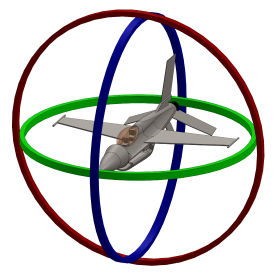
\includegraphics[width=\textwidth]{figs/gimbal}
\caption{3-Axis gimbal}
\label{fig:gimbal}
\end{subfigure}
\begin{subfigure}{0.5\textwidth}
\centering
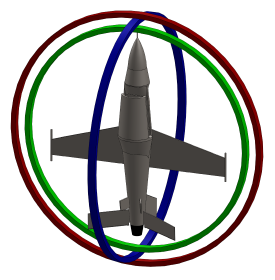
\includegraphics[width=\textwidth]{figs/gimbal-lock}
\caption{Locked gimbal with loss of DOF}
\label{fig:gimbal-lock}
\end{subfigure}
\caption{Gimbal lock}
\end{figure} 
\par
What is clear in a physical system is not necessarily as clear mathematically. An obvious loss of differentiability is manifested in the Euler Matrix $\Psi(\eta)$, Eq:\ref{eq:angular-rates.e} from Section:\ref{subsec:proto.conventions.frames}. The relation between angular velocity, in the inertial frame or inversely in the body frame, and the angular rates of the Euler Angles.
\begin{equation}\label{eq:euler-derivative}
\begin{bmatrix}
\dot{\phi}\\
\dot{\theta}\\
\dot{\psi}
\end{bmatrix}
=\begin{bmatrix}
1 & sin(\phi)tan(\theta) & cos(\phi)tan(\theta)\\
0 & cos(\phi) & -sin(\phi)\\
0 & sin(\phi)sec(\theta) & cos(\phi)sec(\theta)\\
\end{bmatrix}
\begin{bmatrix}
p\\
q\\
r
\end{bmatrix}
=\Phi(\eta)\omega_b
\end{equation}
\begin{equation}
\text{As}~\underset{{\theta \rightarrow \pi /2}}{lim}~sec(\theta),tan(\theta)\rightarrow \infty
\end{equation}
Or that $\Phi(\eta)$ is undefined at $\theta=\pi/2$. 
It's clear to see that in Eq:\ref{eq:euler-derivative} there exists an undefined singularity as $\theta\rightarrow\pi/2$. The physical consequence of this is the loss of a degree of freedom. More specifically, if one looks at how the Z-Y-X rotation (or transformation) matrices are formulated:
\begin{subequations}
\begin{equation}
\mathbb{R}_I^b = \mathbb{R}_z\mathbb{R}_y\mathbb{R}_x=\begin{bmatrix}
c_\psi & -s_\psi & 0\\
s_\psi & c_\psi & 0\\
0 & 0 & 1
\end{bmatrix}
\begin{bmatrix}
c_\theta & 0 & s_\theta\\
0 & 1 & 0\\
-s_\theta & 0 & c_\theta
\end{bmatrix}
\begin{bmatrix}
1 & 0 & 0\\
0 & c_\phi & -s_\phi\\
0 & s_\phi & c_\phi
\end{bmatrix}
\end{equation}
\begin{equation}
\mathbb{R}_I^b=\begin{bmatrix}
c_\psi c_\theta & c_\psi s_\theta s_\phi - s_\psi c_\phi & c_\psi s_\theta c_\phi + s_\psi s_\phi\\
s_\psi c_\theta & s_\psi s_\theta s_\phi + c_\psi c_\phi & s_\psi s_\theta  c_\phi - c_\psi s_\phi\\
-s_\theta & c_\theta s_\phi & c_\phi c_\theta\\
\end{bmatrix}
\end{equation}
In the case where $\theta=\pi/2$, and using trigonometric double angles;
\begin{equation}\label{eq:gimbal}
=\begin{bmatrix}
0 & c_\psi s_\phi - s_\psi c_\phi & c_\psi c_\phi + s_\psi s_\phi\\
0 & s_\psi s_\phi + c_\psi c_\phi & s_\psi c_\phi - c_\psi s_\phi\\
-1 & 0 & 0\\
\end{bmatrix}
=
\begin{bmatrix}
0 & s(\phi - \psi) & c(\phi - \psi)\\
0 & c(\phi - \psi) & s(\phi - \psi)\\
-1 & 0 & 0
\end{bmatrix}=\mathbb{R}_{x'}(\phi-\psi)
\end{equation}
\end{subequations}
Where the resultant in Eq:\ref{eq:gimbal} represents an x-axis rotation in a new intermediate frame, post a 90\textdegree ~rotation in the y-axis. Through trigonometric double angles a degree of freedom is lost at $\theta=\pi/2$, when $\phi$ \& $\psi$ effect the same angle.
%====================================================
\subsection{Quaternion Dynamics}
\label{subsec:dynamics.rigidbody.quaternion}
%====================================================
An algorithm proposed in \emph{How To Avoid a Singularity When Using Euler Angles?}\cite{euleranglesingularity} suggested a solution the problem of Euler Angle singularities. The proposed heuristic was to switch between sequencing conventions (ZYX,ZYZ etc\ldots there are 12 in total) such that the singularity is always avoided. However the implementation of such an algorithm is cumbersome and inefficient. Far more elegant is the use of \emph{quaternion} attitude representations in $\mathbb{R}^4$ (\cite{rotationsequences,quaterniondynamics,spacecraftattitutdequaternions} amongst others\ldots).
\par
A quaternion is analogous to a rotation matrix in that it represents an attitude difference between two reference frames. An $\mathbb{R}^3$ position is paramterized as a single rotation $\theta$ about a unit axis $\hat{u}$ (Sic Rodriguez Formula\cite{unwinding}). Without deliberating too much on their proof or details, a quaternion consists or a scalar component, $q_0$, and complex vector component, $\vec{q}\in \mathbb{C}^3$, such that;
\begin{equation}
Q\triangleq 
\begin{bmatrix}
q_0 \\
\vec{q}
\end{bmatrix}
~~\in\mathbb{R}^4
\end{equation}
The relationship between an Euler Angles rotation matrix $\mathbb{R}_I^b(\eta)$ and a quaternion attitude $Q_b$ is given by the Rodriguez formula:
\begin{equation}\label{eq:rodriguez}
\mathbb{R}_I^b(\eta)=\mathbb{R}(Q_b)=\mathbb{I}+2q_0[\vec{q}~]_\times+2[\vec{q}~]^2_\times
\end{equation}
Any and all quaternions, unless otherwise stated, in this dissertation are all unit quaternions\footnote{Unit quaternions are a subset of the quaternion space}, $Q\in\mathbb{Q}_u$. The need for quaternions with unity magnitude is such to ensure rotational operations don't affect the magnitude of the vector operand. A unit quaternion is defined as:
\begin{equation}
||Q||=\sqrt{{q_0}^2+\vec{q}~^2}=1
\end{equation}
Quaternion multiplication is distributive and associative, but not commutative. Specifically a quaternion multiplciation operation is equivalent to the Hamilton product. For two quaternions, $Q$ \& $P$:
\begin{subequations}
\begin{equation}
Q\otimes P = \begin{bmatrix}
q_0 \\
\vec{q}
\end{bmatrix}
\otimes
\begin{bmatrix}
p_0 \\
\vec{p}
\end{bmatrix}
\end{equation}
\vspace{-5pt}
\begin{equation}
=q_0 p_0 - \vec{q}\cdot \vec{p}+p_0 \vec{q} + q_0 \vec{p} + \vec{q}\times\vec{p}
\end{equation}
\end{subequations}
Seeing that the vector component of a quaternion is complex valued, it is natural that there exists a quaternion conjugate property. Namely:
\begin{equation}
Q^*=\begin{bmatrix}
q_0 \\
-\vec{q}
\end{bmatrix}
\end{equation}
It then follows that\footnote{Disambigation:$\mathbb{I}$ in this context is a $4\times 4$ identity matrix, not an inertial matrix}:
\begin{equation}
Q\otimes Q^* = \mathbb{I}_{4\times 4}
\end{equation}
To apply quaternion rotations to a vector $\vec{v} \in\mathbb{R}^3$ involves multiplication by two unit quaternions. 
\begin{equation}
\begin{bmatrix}
0 \\
\vec{v}~'
\end{bmatrix}
=Q\otimes
\begin{bmatrix}
0 \\
\vec{v}
\end{bmatrix}
\otimes Q^*
\end{equation}
Mostly, the zero scalar components are omitted in a rotation (\emph{or transformation}) operation, such that it is recognized the vector operands are substituted with quaternions.
\begin{equation}\label{eq:quaternion-rotation}
\vec{v}~'=Q \otimes (\vec{v}) \otimes Q^*
\end{equation} 
In the case of rigid body attitude representation, $Q_b$ is the quaternion which represents the difference between $\mathcal{F}^b$ and $\mathcal{F}^I$. A quaternion operator is equivalent to a rotation matrix operation:
\begin{equation}
\mathbb{R}_I^b \underset{Q}{\iff} Q_b \otimes (.) \otimes Q_b^*
\end{equation}
A quaternion time derivative, with $Q_\omega$ being a quaternion with a vector component equal to angular velocity $\omega\in\mathcal{F}^b$ and a zero scalar component, is given by:
\begin{equation}
\frac{d}{dt}Q_b=\frac{1}{2}Q_b\otimes Q_{\omega}=\begin{bmatrix}
-\frac{1}{2}\vec{q}^{~T} \vec{\omega}_b\\
\frac{1}{2}\big([\vec{q}~]_\times+q_0\mathbb{I}\big)\vec{\omega}_b
\end{bmatrix}
\end{equation}
Using quaternions to represent attitudes negates the need for an Euler Matrix, $\Phi(\eta)$, to represent attitudes and their rates. A body quaternion is fully defined in the body frame. The first quaternion time derivative replaces Eq:\ref{eq:states.a}\& Eq:\ref{eq:states.c};
\begin{subequations}
\begin{equation}
\dot{\mathcal{E}}=\mathbb{R}_b^I(-\eta)\vec{\nu}\underset{Q}{\iff}Q_b\otimes\vec{\nu}\otimes Q_b^*
\end{equation}
\vspace{-10pt}
\begin{equation}
\dot{\eta}=\Phi(\eta)\vec{\omega}_b\underset{Q}{\iff}\dot{Q}=\frac{1}{2}Q_b\otimes Q_\omega
\end{equation}
\end{subequations}
Second order derivatives for quaternion acceleration aren't as useful as their velocity counterparts. The second order derivative is mentioned here however it's only relevant to quaternion backstepping in the control chapter. If possible, quaternion accelerations are mostly avoided due to their complexity;
\begin{equation}
\ddot{Q}\big(\dot{Q},Q,t)=\dot{Q}\otimes Q^* \otimes \dot{Q}+\frac{1}{2}Q\otimes \big[\mathbb{I}_b^-1(\tau-4(Q^*\otimes \dot{Q})\times(\mathbb{I}_b(Q^*\otimes \dot{Q}))\big]
\end{equation}
%====================================================
\subsection{Quaternion Unwinding}
\label{subsec:dynamics.rigidbody.unwinding}
%====================================================
Although quaternions are better than Euler angles and lack the associated singularity, they do contain one caveat. Seeing that a quaternion $Q=[q_0~\vec{q}~]^T$ represents an attitude orientation of a body in $\mathbb{R}^3$ using $\mathbb{R}^4$ variables there exists what is called dual coverage\cite{unwinding}.
Each unit quaternion, stemming from Euler-Rodriguez theorem, is parametrized such that the quaternion operation represents an eigenaxis rotation of $\theta$ about an axis $\hat{u}$ such that:
\begin{equation}
Q=\begin{bmatrix}
q_0\\
\vec{q}
\end{bmatrix}=
\begin{bmatrix}
cos(\theta/2)\\
sin(\theta/2)\hat{u}
\end{bmatrix}
\end{equation}
That rotation is executed through the quaternion operator Eq:\ref{eq:quaternion-rotation}. As a result its clear to see that for each unique attitude in 3-Dimensions there exist two quaternions which correlate to the same position. Namely:
\begin{subequations}
\begin{equation}
Q =
\begin{bmatrix}
q_0 \\
\vec{q}
\end{bmatrix}
=
\begin{bmatrix}
cos(\theta/2)\\
sin(\theta/2)\hat{u}
\end{bmatrix}
.
\end{equation}
And seeing that $\theta=2\pi-\theta$, then;
\begin{equation}
Q=\begin{bmatrix}
cos(\pi - \theta/2)\\
sin(\pi - \theta/2)\hat{u}
\end{bmatrix}
=
\begin{bmatrix}
-cos(\theta/2)\\
sin(\theta/2)\hat{u}
\end{bmatrix}
\end{equation}
\end{subequations}
Every physical attitude in $\mathbb{R}^3$ has two corresponding quaternions in $\mathbb{R}^4$; $[\pm q_0~\vec{q}~]^T$. A consequence of this is two possible error state trajectories for every attitude difference. A clockwise $\theta$ rotation and an anticlockwise $2\pi-\theta$ negative rotation. This could lead to an erroneous and unnecessary "unwinding" of a complete counter revolution as a result of a dual covered error state. 
\par
Often the sign scalar component of the attitude quaternion error (Section:\ref{subsec:control.attitude.quaternion}) is simply neglected or assumed positive. As such for attitude controllers the requirement is that for positive and negative scalars the control input is consistent:
\begin{equation}
\nu_d=h([q_0~\vec{q}~]^T,t)=h([-q_0~\vec{q}~]^T,t)
\end{equation}
Or more simply that $Q_e=[|q_0|~\vec{q}~]^T$. The most simple solution which adheres to that constraint is to simply neglect the scalar component and use $h(\vec{q}_e,t)$. A positive quaternion scalar will always ensure that an error state represents a right-handed clockwise rotation. If the resolution of trajectory co-ordinates generated is sufficiently high enough, the control plant will never encounter a problem.
\par
One proposal in \emph{Nonlinear Quadcopter Attitude Control}\cite{nonlinearquadcopter} suggested using a \emph{signum} operator to design the signs of the controller coefficients for the virtual control plant input. 
\begin{subequations}\label{eq:signum-unwinging}
\begin{equation}
\vec{omega}_d=\frac{2}{\tau}sgn(q_0)\vec{q}
\end{equation}
\vspace{-10pt}
\begin{equation}
sgn(\vec{q})=
\begin{cases}\begin{array}{ll}
1 & ~~\vec{q}\geq 0\\
-1 & ~~\vec{q}< 0\\
\end{array}
\end{cases}
\end{equation}
\end{subequations}
The resultant \emph{hybrid} controller provides global asymptotic stability, but only in the case that the eigenaxis angle $\theta\leq 180$\textdegree~. The control law described in Eq:\ref{eq:signum-unwinging} would still need the control torques to be designed from the angular velocity virtual control input.
\par
An alternative proposal \cite{unwinding} was to lift the quaternion error-state back into $\mathbb{R}^3$ using the Rodriguez formula, Eq:\ref{eq:rodriguez}. The mapping back to $\mathbb{R}^3$ effectively ensures that $\theta$ is minimized, or that the error-state imposes the shortest possible rotation between the reference and desired body frames.
%====================================================
\section{Multibody Nonlinearities}
\label{sec:dynamics.nonlinearities}
%====================================================
The inertial equations presented first are all consequences of design decisions taken. As a result they're an extension of the design in Chapter:\ref{sec:proto.design} but are pertinent to the following nonlinear multibody dynamics derived here. Although inertias are presented here rounded to either 2 or 0 decimal places, full floating point numbers are used in simulation and prototype software.
%====================================================
\subsection{Inertial Matrices \& Masses}
\label{subsec:dynamics.nonlinearities.inertia}
%====================================================
\subsubsection*{Inertias}
An undesirable side effect of the relative rotations within a non-rigid body are the inertial responses associated with such movements. Given Newton's Second Law of Rotational Motion$^{\dagger}$, each applied rotation is going to produce an equal but opposite reaction onto the principle inducing frame. Similarly a gyroscopic cross product from rotational velocities is also present. Such first and second order effects are often neglected given that the angular rates which they're dependent on are mostly small enough to approximate as zero, $\vec{\omega}_b\approx\vec{0}$. A dynamic set-point (non-zero) attitude tracking plant is, however, going to produce sizable time varying body angular velocities and accelerations. Unlike a traditionally actuated quadrotor, such effects have to be accounted for.
\begin{figure}[htbp]
\centering
\begin{subfigure}{0.49\textwidth}
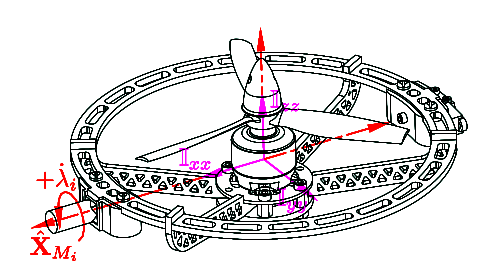
\includegraphics[width=\textwidth]{figs/inertia-inner}
\caption{Inner Ring Rotational Structure}
\label{fig:inertia-inner}
\end{subfigure}
\begin{subfigure}{0.49\textwidth}
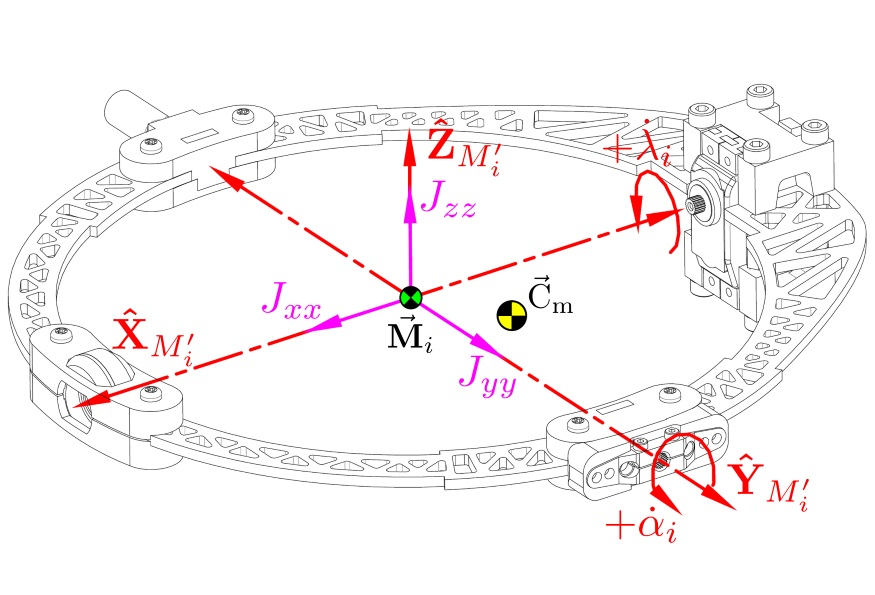
\includegraphics[width=\textwidth]{figs/inertia-middle}
\caption{Middle Ring Rotational Structure}
\label{fig:inertia-middle}
\end{subfigure}
\caption{Inertial Measurement References}
\end{figure}
\par
The manifestation of those responses are explored next in Section:\ref{subsec:dynamics.nonlinearities.gyrotorques}. Both of those effects are dependent on the rotational body's inertial tensor\footnote{All inertias are assumed symmetrical and calculated in SolidWorks with overridden masses to match physical prototype measurements, all those values are included in Appendix:\ref{app:bom}} about each respective rotational axis. The magnitude of those inertias are obviously a by-product of the structure's design. Starting with the innermost assembly, in each Motor Frame $\mathcal{F}^{M_i}$, the inner ring structure is a 92g body (all components incorporated). The rotational center \emph{roughly} coincides with the center of its mass ($C.M=[-1.44~~0~~5.81]^T~~[mm]$ relative to its rotational center). The inner ring being rotated by $\lambda_i$ about the $\hat{X}_{M_i}$ axis then has an inertial matrix (centered and aligned with axes as in Fig:\ref{fig:inertia-inner}):
\begin{subequations}\label{eq:inertia.inner}
\begin{equation} \label{eq:inertia.inner.a}
\mathbb{I}_{M_i}=\begin{bmatrix}
561.96 & -32.29	& -0.26\\
-32.29 & 1888.74 & 0.00\\
-0.26 & 0.00	& 2090.97\\
\end{bmatrix}~~~[g.cm^2]
\end{equation}
\vspace{-5pt}
\begin{equation} \label{eq:inertia.inner.b}
\approx diag\big(562, ~1889, ~2091\big)\times10^{-7}~~~[kg.m^2]
\end{equation}
\end{subequations}
The effect of rapidly spinning propellers on the inertia in Eq:\ref{eq:inertia.inner.a} is approximated well by a solid disc, hence the inner ring's inertial components are regarded as constant. The moment of inertia about that $\hat{X}_{M_i}$ rotational axis, pertinent to a $\lambda_i$ rotation, is then $\mathbb{I}_{\lambda}\approx 531\times10^{-7}~~[kg.m^2]$.
\par
The first $\lambda_i$ actuating servo and bearing supports are affixed to the intermediate middle ring assembly (Fig:\ref{fig:inertia-middle}). The middle ring frame, $\mathcal{F}^{M_i'}$, is a $98g$ body, excluding the inner most ring. Collectively the mass for both the inner and middle rings assemblies is $m_{module}=190g$. The middle ring is rotated by $\alpha_i$ about its $\hat{Y}_{M_i'}$ axis. The compound body's inertia about that axis of rotation, $\hat{Y}_{M_i}$, is a combination of both the middle ring's inertia and the inner ring's.  The latter contribution being a function of the \emph{rotation} (not transformation) angle $\lambda_i$ which, from the conservation of angular momentum theory \cite{rigidbodyinertia}\footnote{$\mathbb{R}_x$ is a full rank and square, so an inverse $\mathbb{R}^{-1}_{x}$ always exists.}, is:
\begin{subequations}\label{eq:inertia.middle}
\begin{equation} \label{eq:inertia.middle.a}
\text{If} ~~\mathbb{I}_{middle}=\begin{bmatrix}
2905.70 & 0.02 & 390.89\\
0.02 & 8446.41 & 0.01\\
390.89 & 0.01 & 11125.74\\
\end{bmatrix}~~~[g.cm^2]
\end{equation}
\vspace{-5pt}
\begin{equation}\label{eq:inertia.middle.b}
\mathbb{I}_{M_i'}=\mathbb{I}_{middle}+\mathbb{R}_{x}(\lambda_i)\big(\mathbb{I}_{inner}\big)\mathbb{R}_{x}^{-1}(\lambda_i)
\end{equation}
\vspace{-10pt}
\begin{equation}\label{eq:inertia.middle.c}
\mathbb{I}_{M_i'}(\lambda_i)=\mathbb{I}_{const}+\mathbb{I}_{M_i}(\lambda_i)
\end{equation}
\vspace{-10pt}
\begin{equation} \label{eq:inertia.middle.d}
\approx\begin{bmatrix}
3468 & 0 & 391\\
0 & 10436 & 0\\
391 & 0 & 13155\\
\end{bmatrix}
+
\begin{bmatrix}
0 & -32{c}_{\lambda} & -32{s}_{\lambda}\\
-32{c}_{\lambda} & -101{c}_{2\lambda} & 101s_{2\lambda}\\
-32{s}_{\lambda} & 101s_{2\lambda} & 101{c}_{2\lambda}\\
\end{bmatrix}
\times10^{-7}~~~[kg.m^2]
\end{equation}
\end{subequations}
With $\mathbb{I}_{inner}=\mathbb{I}_{M_i}$ being the inertia from Eq:\ref{eq:inertia.inner.a}, re-orientated through a rotation $\mathbb{R}_x(\lambda_i)$. The net inertia is then a combination of an inertia as a function of the rotation angle $\lambda_i$ and a constant inertia (Eq:\ref{eq:inertia.middle.c}), which together are then simplified\footnote{Eq:\ref{eq:inertia.middle.d} is rounded to no decimal places, seeing that its units are already $\times10^{-7}$ and thus some products of inertia are omitted.} to Eq:\ref{eq:inertia.middle.d}. It's important to note the two non-zero products of inertia, $\mathbb{I}_{yx}$ and $\mathbb{I}_{yz}$, which are going to result in a vector torque $\vec{\tau}_\eta$ response. The inertia then encountered by an $\alpha_i$ rotation is:
\begin{equation}\label{eq:inertia.middle.vpa}
\mathbb{I}_\alpha(\lambda)\approx[-32{c}_{\lambda},~ 10436-101{c}_{2\lambda},~ 101{s}_{2\lambda}]^T\times10^{-7}~~~[kg.m^2]
\end{equation}
\par
Variable inertias dependent on state input variables are the first of many non-trivial aspects unique to this aircraft's design. The resultant control solutions are thus decidedly plant dependent in their formulation. Secondly, the center of mass for the motor module's compound assembly isn't coincidental with either rotational axes intersection. As a result the effective center of mass for the entire structure is going to be a function of the angular rotational position of each motor module and time varying.
\par
\begin{figure}[htbp]
\centering
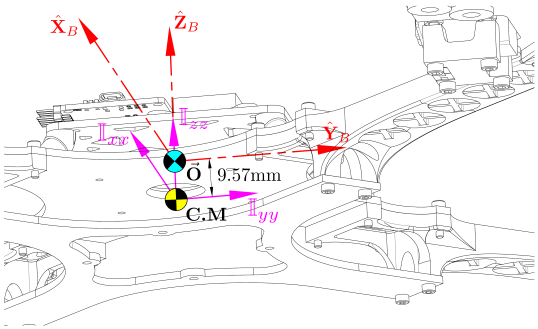
\includegraphics[width=0.8\textwidth]{figs/inertia-center}
\caption{Body Frame Center of Mass}
\label{fig:inertia-center}
\end{figure}
The second $\alpha_i$ rotating servo adjoins the complete motor module (both the inner and middle ring assemblies) to the body structure. The inertial volume of the servo and bearing supports contribute then to the body structure's inertia, whose value excludes any of the four motor modules. Consisting of servo and bearing damping brackets, each "damping" assembly collectively weighs $84g$ and suspends the motor modules from the body frame with a set of silicon damping balls. The body structure's center of mass (without motor modules, Fig:\ref{fig:inertia-center}) coincides with the XY directional axes and lies $\Delta Z=-9.57~mm$ below the Body Frame's origin of motion, $\vec{O}\in\mathcal{F}^b$.
\\
\emph{\color{Gray}Note: the origin which all motion is calculated with respect to is co-planar to the motor module's rotational centers, \underline{not} the net center of mass.}
\\
The body's weight, including all four damping assemblies and electronics, totals to $814.7~g$. The body's net inertia (\emph{sans} motor modules) $\mathbb{I}_{body}$, about its center of mass is (Fig:\ref{fig:inertia-center})
\begin{subequations}\label{eq:inertia.body}
\begin{equation}\label{eq:inertia.body.a}
\mathbb{I}_{body}=\begin{bmatrix}
181689.67 & -0.44 & -8.86\\
-0.44 & 181567.22 &	-19.44\\
-8.86 & -19.44 & 360077.58\\
\end{bmatrix}\times 10^{-7}~~~[kg.m^2]
\end{equation}
Using the Parallel Axis theorem$^{\dagger}$, that same net body inertia about the body frame's origin, $\vec{O}_b$, is:
\begin{equation}\label{eq:inertia.body.b}
{\mathbb{I}_{body}}'=\mathbb{I}_{body}+m(\vec{d}\cdot\vec{d}+\vec{d}\otimes\vec{d})\approx\mathbb{I}_{body}+md^2
\end{equation}
\emph{\color{Gray}Here $\otimes$ represents the Hamilton product of two 3X3 matrices, it's used elsewhere to indicate the quaternion multiplication operator.}
\begin{equation}\label{eq:inertia.body.c}
\underset{\vec{\mathbf{O}}}{{\mathbb{I}_{body}}'}=\begin{bmatrix}
182435.66 & -0.42 & -6.46\\
-0.42 & 182313.18 & -14.52\\
-6.46 & -10.41 & 360077.62\\
\end{bmatrix} \times10^{-7}~~~[kg.m^2]
\end{equation}
\end{subequations}
Net inertia for the compound assembly, $\mathbb{I}_b$\footnote{Disambiguation: $\mathbb{I}_b$ is \emph{net} body frame's inertia, different from $\mathbb{I}_{body}$ which is the inertia for \emph{just} the body structure}, about the origin $\vec{O}_b$ is a combination of all the relative attached bodies. That being; the four motor modules, transformed and then translated to the body origin, and the body structure itself. That transformation is analogous to that of Eq: \ref{eq:motor-module-rotation}. Reiterating that the the origin is co-planar to the module's center of rotation, each motor module's inertia, $\mathbb{I}_{M_i'}$\footnote{As defined in Eq:\ref{eq:inertia.middle.d}}, is further rotated by $\alpha_{i}$ about $\hat{Y}_{M_i'
}$ and finally an orthogonal $\hat{Z}_{M_i''}$ rotation (aligned with $\hat{Z}_b$) onto $\mathcal{F}^b$. Still measured with respect to their individual rotational centers, $\vec{\mathbf{M}}_i$, but re-orientated to align with $||\vec{\mathbf{O}}_b$. Contribution of each motor module's inertia, with $\mathbb{R}_z$ being the same as Eq:\ref{eq:motor-module-rotation.b}, is then:
\begin{subequations}\label{eq:module-inertia}
\begin{equation}\label{eq:module-inertia.a}
\mathbb{I}_{i^{th} motor}=\mathbb{R}_{z}(\sigma_i)\mathbb{R}_{z}(\alpha_i)\big(\mathbb{I}_{M_i'}(\lambda_i)\big)\mathbb{R}^{-1}_{y}(\alpha_i)\mathbb{R}^{-1}_{z}(\sigma_i)
\end{equation}
Expanding that to inner and middle ring components:
\begin{equation}\label{eq:module-inertia.b}
=\mathbb{R}_{z}\mathbb{R}_{y}(\alpha_i)\big(\mathbb{I}_{middle}\big)\mathbb{R}^{-1}_{y}(\alpha_i)\mathbb{R}^{-1}_z+\mathbb{R}_{z}\mathbb{R}_{y}(\alpha_i)\mathbb{R}_{x}(\lambda_i)\big(\mathbb{I}_{inner}\big)\mathbb{R}^{-1}_{x}(\lambda_i)\mathbb{R}^{-1}_{y}(\alpha_i)\mathbb{R}^{-1}_z
\end{equation}
\vspace{-10pt}
\begin{equation}\label{eq:module-inertia.c}
\text{With axes}~\hat{X}\in\mathcal{F}^{M_i},~~\hat{Y}\in\mathcal{F}^{M_i'},~~\hat{Z}\in\mathcal{F}^{M_i''}
\end{equation}
\end{subequations}
\emph{\color{Gray}It's at this stage that, despite simplifications, the symbolic inertial equations all become overly cumbersome to include with numeric values\ldots For the sake of brevity, exact calculated inertial values for the input dependent plant are omitted.}
\par
\begin{figure}[hbtp]
\centering
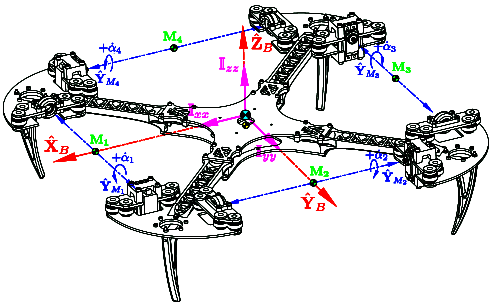
\includegraphics[width=\textwidth]{figs/inertia-frame}
\caption{Inertial Center \& Mass Center}
\label{fig:inertia-frame}
\end{figure}
Each module's rotational center ($[\pm 195.16~~0~~0]$ \& $[0~~\pm 195.16~~0]$ recalling Fig:\ref{fig:body-frame}) are spaced equally relative to $\vec{\mathbf{O}}_b$ with a parallel axis arm $\vec{L}_{arm}=\begin{bmatrix}
195.16 & 0 & 0
\end{bmatrix}^T~~[mm]$ (Fig:\ref{fig:inertia-frame}). The net inertial equation about $\vec{\mathbf{O}}_b$, dependent on the actuator suite $\mathbb{U}$ positions, can be calculated as:
\begin{subequations}
\label{eq:body-inertia}
\begin{equation}\label{eq:body-inertia.a}
\underset{u\in\mathbb{U}}{\mathbb{I}_b(u)}=\mathbb{I}_{body}+\sum_{i=1}^{4}\mathbb{M}_{i}~~~[kg.m^2]
\end{equation}
\vspace{-10pt}
\begin{equation}\label{eq:body-inertia.b}
\mathbb{M}_i=\mathbb{I}_{i^{th}motor}+m_{module}\big(\vec{L} \cdot \vec{L} - \vec{L}\otimes\vec{L}\big)
\end{equation}
\end{subequations}
Although Eq:\ref{eq:body-inertia} does indeed produce the net body's inertia, the transformations to calculate $\mathbb{M}_i$ are compounded. Motor module inertias are first translated to their centers of rotation from their respective center of masses and then finally to the body frame's origin. Subsequent transformations are successively going to deteriorate the floating point precision of the resultant inertial tensor. Transforming inertial tensors about each sub-body's center of mass directly to the body frame origin will improve the reliability of the produced inertial equations. It is perhaps more intuitive to consider each sub-body's contribution individually, despite having been derived as combined inertial systems previously. 
\begin{equation}\label{eq:body-net}
\underset{u\in\mathbb{U}}{\mathbb{I}_b(u)}=\mathbb{I}_{body}+\sum_{i=1}^{4} \mathbb{M}_{inner}+\sum_{i=1}^{4} \mathbb{M}_{middle}
\end{equation}
\par
The relative movement pertinent to Eq:\ref{eq:inertia.inner} and Eq:\ref{eq:inertia.middle} are separate from those affecting Eq:\ref{eq:body-inertia}. For each inner ring, W.R.T its center of mass measured relative to its center of rotation, different from Eq:\ref{eq:inertia.inner.a}, the inner ring's inertia is calculated as;
\begin{subequations}
\label{eq:body-net-inner}
\begin{equation}
m_{inner}=92~~[g]
\end{equation}
\vspace{-10pt}
\begin{equation}
\underset{C.M}{\mathbb{I}_{inner}}=\begin{bmatrix}
530.88 & -32.29 & 7.46\\
-32.29 & 1855.74 & 0\\
7.46 & 0 & 2088.87\\
\end{bmatrix}~~[g.cm^2]
\end{equation}
\vspace{-5pt}
\begin{equation}
C.M_{inner}=\begin{bmatrix}
-1.44 & 0 & 5.81
\end{bmatrix}^T~~[mm]
\end{equation}
\vspace{-10pt}
\begin{equation}\label{eq:body-net-inner.d}
{C.M_{inner}}'=\mathbb{R}_z\mathbb{R}_y(\alpha_i)\mathbb{R}_x(\lambda_i) \big(C.M_{inner}\big)
\end{equation}
\vspace{-10pt}
\begin{equation}
\underset{||~\vec{\mathbf{O}}}{\mathbb{I}_{inner}}=\mathbb{R}_z\mathbb{R}_y(\alpha_i)\mathbb{R}_x(\lambda_i)\big(\mathbb{I}_{inner}\big)\mathbb{R}^{-1}_x(\lambda_i)\mathbb{R}^{-1}_y(\alpha_i)\mathbb{R}^{-1}_z
\end{equation}
\vspace{-10pt}
\begin{equation}
\Delta L = \vec{L}_{arm}-{C.M_{inner}}'
\end{equation}
\vspace{-10pt}
\begin{equation}
\mathbb{M}_{inner}=\underset{\vec{\mathbf{O}}}{\mathbb{I}_{inner}}=\underset{||~\vec{\mathbf{O}}}{\mathbb{I}_{inner}}+ m_{inner} \big((\Delta L \cdot \Delta L)\mathbb{I}_{3x3} - \Delta L \otimes \Delta L \big)
\end{equation}
\end{subequations}
Similarly for the middle rings:
\begin{subequations}
\label{eq:body-net-middle}
\begin{equation}
m_{middle}=98~~[g]
\end{equation}
\vspace{-10pt}
\begin{equation}
\underset{C.M}{\mathbb{I}_{middle}}=\begin{bmatrix}
2879.06 & 172.29 & 223.58\\
172.29 & 6268.97 & 13.33\\
223.58 & 13.33 & 8947.52\\
\end{bmatrix}~~[g.cm^2]
\end{equation}
\vspace{-5pt}
\begin{equation}
C.M_{middle}=\begin{bmatrix}
-47.00 & 3.74 & -3.63
\end{bmatrix}^T~~[mm]
\end{equation}
\vspace{-10pt}
\begin{equation}\label{eq:body-net-middle.d}
{C.M_{middle}}'=\mathbb{R}_{z}\mathbb{R}_{y}(\alpha_i)\big(C.M_{middle}\big)
\end{equation}
\vspace{-10pt}
\begin{equation}
\underset{||\vec{\mathbf{O}}}{\mathbb{I}_{middle}}=\mathbb{R}_z\mathbb{R}_y(\alpha_i)\big(\mathbb{I}_{middle}\big)\mathbb{R}^{-1}_y(\alpha_i)\mathbb{R}^{-1}_z
\end{equation}
\vspace{-10pt}
\begin{equation}
\Delta L = \vec{L}_{arm}-{C.M_{middle}}'
\end{equation}
\vspace{-10pt}
\begin{equation}
\mathbb{M}_{middle}=\underset{\vec{\mathbf{O}}}{\mathbb{I}_{middle}}=\underset{||\vec{\mathbf{O}}}{\mathbb{I}_{middle}}+m_{middle}\big((\Delta L\cdot\Delta L)\mathbb{I}_{3x3}-\Delta L \otimes \Delta L \big)
\end{equation}
\end{subequations}
Unless otherwise specified; any inertia $\mathbb{I}_b(u)$, irrespective of arguments, will refer to an instantaneous calculated solution to Eq:\ref{eq:body-net} given a particular $u(t)\in\mathbb{U}$. The purpose of the derivations Eq:\ref{eq:body-net-inner} \& Eq:\ref{eq:body-net-middle} is twofold; highlighting both the inertial contributions and the variable center of masses for each sub-body. Seeing that the origin of the motion frame $\mathcal{F}^b$ and the net body's center of mass aren't coincidental, it's important to quantify the equation for the varying center of mass. If, for a collection of $n$ bodies, with each body's center $\vec{X}_i$ and a mass $m_i$, the net center of mass is:
\begin{subequations}
\label{eq:mass-center}
\begin{equation}\label{eq:mass-center.a}
C.M = \frac{\sum_{i=1}^{n} m_i.\vec{X}_i}{\sum_{i=1}^{n} m_i}
\end{equation}
Such that, with $\vec{X}_{inner}$ \& $\vec{X}_{middle}$ being rotated centers of mass defined in Eq:\ref{eq:body-net-inner.d} \& Eq:\ref{eq:body-net-middle.d} respectively, the entire assembly has a center of mass$^{\dagger}$:
\begin{equation}\label{eq:mass-center.b}
C.M(u)=\frac{m_{body}.\vec{X}_{body}+\sum m_{inner}.\vec{X}_{inner}+\sum m_{middle}.\vec{X}_{middle}}{m_{body}+\sum m_{inner} + \sum m_{middle}}
\end{equation}
Making the resultant gravitational torque\footnote{With $\vec{G}_b=\mathbb{R}_I^b\vec{F_g}~~[N]$} about the origin $\vec{\mathbf{O}}$ at any given moment:
\begin{equation}
\Delta C.G = \vec{\mathbf{O}}-C.M
\end{equation}
\vspace{-20pt}
\begin{equation}
\tau_g=\Delta C.G\times\vec{G}_b ~~~[N.m],\tau_g\in\mathcal{F}^b
\end{equation}
\end{subequations}
The net mass for the whole assembly is 1574 g. For reference the center of gravity when all actuators are at their zero positions is: $[-0.02~-0.03~-4.5]~~[mm]$. Then, according to Eq:\ref{eq:body-net}, the inertial tensor for the net assembly at the rest conditions, $u=\vec{0}$, about the origin $\vec{\mathbf{O}}$ is:
\begin{equation}
\mathbb{I}_b(\vec{0})=\begin{bmatrix}
317784.78 & -0.42 & -6.46\\
-0.42 & 317662.31 & -14.52\\
-6.46 & -14.52 & 628430.75\\
\end{bmatrix}
~~[g.cm^2]
\end{equation}
%====================================================
\subsection{Relative Rotational Inertia \& Gyroscopic Torques}
\label{subsec:dynamics.nonlinearities.gyrotorques}
%====================================================
One of the biggest sources of non-linear disturbance for a multi-body system is its inertial response from relative interactions within the assemblage. The induced torque responses to the relative rotations, the only permissible relative motion, between each connected rigid body are transferred from interacting bodies as a result of Newtons second law of rotational motion. For each of the motor modules pitching or rolling motion, the servo motors generate a torque to induce that rotation. Opposed to that rotation are both inertial and gyroscopic response(s) of that body being acted upon. The latter being a consequence of a vector's time derivative in a rotating frame, Eq:\ref{eq:reynolds}.
\par
Each of the four motor modules are symmetrical and as such the induced torque response characteristics for one module can be extrapolated through a reference frame rotation. Seeing that each relative rotation from the actuator set $u\in\mathbb{C}$ is induced independently and upon a different body, their responses are calculated separately too. Drawing again from Lagrangian theory\footnote{Generalized linear kinetic energy is considered on the whole body separately} the rotational kinetic energy for the inner ring assembly $\mathcal{F}^{M_i}$ is:
\begin{equation}
\mathcal{L}_{M_i}=\frac{1}{2}\vec{\Omega}_i^{~T}\big(\mathbb{I}_{prop}\big)\vec{\Omega}_i+\frac{1}{2}\vec{\lambda}_i^{~T}\big(\mathbb{I}_{Inner}\big)\vec{\lambda}_i
\end{equation}
And noting that $\vec{\Omega}_i=[0~~0~~\Omega_i]^T\in\mathcal{F}^{M_i}$ and 

%====================================================
\subsection{Coriolis Acceleration}
\label{subsec:dynamics.nonlinearities.coriolis}
%====================================================

%====================================================
\section{Aerodynamics}
\label{sec:dynamics.aero}
%====================================================
\subsection{Thrust Forces}
\label{subsec:dynamics.aero.bem}
%====================================================
\subsection{Propeller Torques}
\label{subsec:dynamics.aero.torque}
%====================================================
\subsection{Drag}
\label{subsec:dynamics.aero.drag}
%====================================================
\subsection{Hinged Propeller Conning \& Flapping}
\label{subsec:dynamics.aero.flap}
%====================================================
\subsection{Vortex Ring State}
\label{subsec:dynamics.aero.vrs}
%====================================================

%====================================================
\section{Consolidated Model}
\label{sec:dynamics.model}%====================================================